\documentclass[a4paper,11pt,oneside]{article}
\pagestyle{plain}
%\usepackage[a4paper, margin=1.2in]{geometry}

\usepackage{mdframed}

%configuración del idioma y la codificacion
\usepackage[spanish]{babel}
\usepackage[utf8x]{inputenc}
\usepackage[T1]{fontenc}

%fuente
%\usepackage{times}
\usepackage{palatino}

%math
\usepackage{amsmath,amssymb}
\usepackage{amsthm}
\usepackage{bbold}
\usepackage{dsfont}
\usepackage{braket,mleftright}

\usepackage{graphicx}
\usepackage{subcaption}

%otros paquetes
%\usepackage{rotating}
\usepackage{cite}
\usepackage[linktoc=page]{hyperref}
\usepackage{indentfirst}

%comandos
\newcommand{\mean}[1]{\langle #1 \rangle}

\title{Práctica computacional - Modelo de Ising}
\author{}
\date{}

\begin{document}
\maketitle

\section{Introducción}
Consideremos una grilla de $N = L\times L$ sitios en cada uno de los cuales hay
un spin que solo puede tomar los valores $S = 1,-1$. Estos
spines tienen interacciones tipo Ising dadas por el siguiente Hamiltoniano:
\begin{equation}
    H = -J\sum_\text{n.n} S_i S_j - B \sum_i S_i
\end{equation}
Donde la primer suma es sobre primeros vecinos y $J$ y $B$ son parámetros que
dan la energía de interacción entre spines, entre cada uno de ellos y un
campo magnético externo. Supongamos que queremos calcular numéricamente algún
observable macroscópico a una dada temperatura $\beta^{-1}$, como por ejemplo
el valor medio de la magnetización total:
\begin{equation}
    \mean{M} = \sum_{S_1,\dots,S_N} p_{S_1,\dots,S_N} \; (S_1+S_2+\dots+S_N).
    \label{eq:mag_total}
\end{equation}
Esta vez la suma es sobre todas las configuraciones posibles de los spines, y
$p_{S_1,\dots,S_N}$ es la probabilidad de cada configuración, que según el
ensamble canónico, es:
\begin{equation}
    p_{S_1,\dots,S_N} = \frac{1}{Z} \; e^{-\beta H(S_1,\dots,S_N)},
\end{equation}
donde $Z$ es la función de partición:
\begin{equation}
    Z = \sum_{S_1,\dots,S_N} e^{-\beta H(S_1,\dots,S_N)}.
\end{equation}
Si quisieramos evaluar la fórmula de la ecuación \ref{eq:mag_total} tal cual esta planteada,
necesitariamos recorrer todos los estados posibles del sistema (al igual que
para calcular exactamente la función de partición, necesaria para calcular las
probabilidades $p_{S_1,\cdots,S_N}$). El problema es que la cantidad de estados
es $2^{N}$, y solo para $N=100$ este número es ridículamente grande. Ninguna
computadora podría recorrer todos estos estados en un tiempo razonable. Pero,
como sabemos, hacer eso tampoco es necesario, ya que solo una fracción de los
estados posibles contribuirá apreciablemente a la suma en la ecuación
\ref{eq:mag_total}. Entonces, dado que no podemos recorrer todos los estados,
una estrategia posible sería solo considerar algunos términos de la ecuación
\ref{eq:mag_total}, de una forma tal que estos términos sean representativos
de los estados que típicamente recorre el sistema cuando se encuentra a
temperatura $\beta^{-1}$. Estos términos, naturalmente, son aquellos para los
cuales la probabilidad $p_{S_1,\dots,S_N}$ es mayor.
Dicho de otra forma, necesitamos `muestrear' la
distribución de probabilidad $p_{S_1,\dots,S_N}$, es decir generar estados de
forma tal que la fracción de veces que se genera el estado $(S_1,\dots,S_N)$
sea $p_{S_1,\dots,S_N}$. El algoritmo de Metrópolis, que pertenece a la familia
mas general de algoritmos de Montecarlo, es una solución a este problema.

\section{Algoritmo de Metrópolis}

El algoritmo de Metrópolis genera estados secuencialmente, de forma que cada
estado es generado a partir del anterior de forma estocástica. La secuencia de
estados generados es entonces una cadena de Markov, y el proceso de generación
es tal que la distribución estacionaria es la distribución de Boltzmann que se
desea muestrear. El algoritmo es muy sencillo, y para el caso de un sistema de
Ising 2D se describe de la siguiente manera:
\begin{enumerate}
\item Se selecciona un estado inicial al azar o con algún criterio. Este estado
    se uarda en una matriz $S$ de $L\times L$ cuyos elementos son $1$ o $-1$.
\item Se elige aleatoriamente un sitio de la red. Es decir se eligen
    coordenadas $i$ y $j$ según una distribución uniforme entre $1$ y $L$ (o
    entre $0$ y $L-1$, según como se indexen las matrices en el lenguaje que
    usen)
\item Se calcula la diferencia de energía $\Delta E$ que resultaría de invertir
    el estado del spin en la posición $(i,j)$.
\item Si $\Delta E \leq 0$, se invierte el spin, es decir que el nuevo estado
    de la red, $S'$, es igual a $S$ excepto en el sitio $(i,j)$,
    donde $S'(i,j) = -S(i,j)$.
\item Si $\Delta E >0$, el spin se invierte con probabilidad $p = e^{-\beta\Delta
    E}$. El nuevo estado de la red es de nuevo $S'$, que con probabilidad
    $1-p$ será igual a $S$, y con probabilidad $p$ sera distinto sólo en el
    valor del sitio $(i,j)$.
\item Se repiten los pasos 2-5 con el nuevo estado $S'$, tantas veces como sea
    necesario.
\end{enumerate}
Este algoritmo genera una secuencia de estados $S_1,S_2,S_3,\dots$, donde cada
estado depende solo del anterior de una manera estocástica (un dado estado
$S_k$ puede dar lugar a muchos estados distintos $S_{k+1}$ con distintas probabilidades).
El punto crucial del algoritmo es que las probabilidades de transición de un
estado $a$ a un estado $b$ satisfacen la condición:
\begin{equation}
    \frac{P(a\to b)}{P(b\to a)} = e^{-\beta(E_b-E_a)} = \frac{e^{-\beta
    E_b}/Z}{e^{-\beta E_a}/Z} = \frac{P_b}{P_a}
    \label{eq:bal_detallado}
\end{equation}
Esta condición se conoce como 'balance detallado', e implica que el proceso
estocástico alcanza un estado estacionario donde la probabilidad de observar el
estado $a$ es $P_a \propto e^{-\beta E_a}$. Notar que en ningún paso del
algoritmo, ni en la condición de balance detallado, es necesario conocer la
constante de normalización de la distribución de probabilidad que se desea
muestrear (en este caso, esta constante es la función de partición canónica).
Por lo tanto, la condición de balance detallado nos asegura que cuando el
proceso de generación de estados alcance un estado estacionario (lo cuál se
espera que suceda luego de un número suficiente de interaciones) la
probabilidad de cada estado estará dada por el factor de Boltzmann. 


\begin{mdframed}
\emph{Ejercicio: Tiempo de equilibración}. Estudie como evoluciona la
magnetización y la energía del sistema en función del número de iteraciones,
comenzando de una configuración aleatoria. ¿Cuántas iteraciones son necesarias
para que estas magnitudes alcancen un equilibrio? ¿Depende este tiempo del
tamaño del sistema o de la temperatura? Como ejemplo se muestra la
magnetización total en función del número de iteraciones para $L=16,T=2,J=1,B=0$.

{\centering 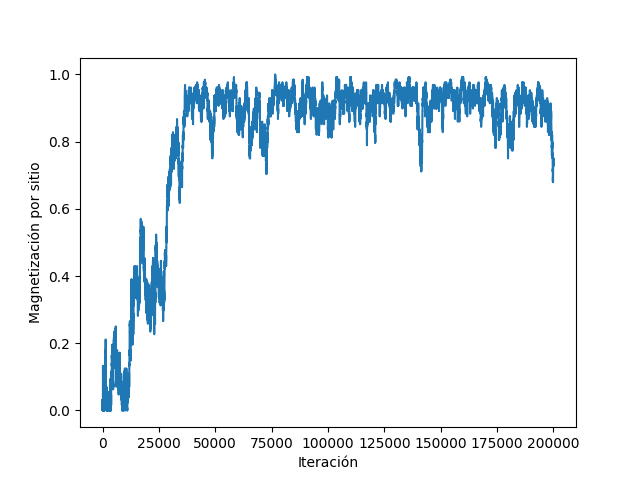
\includegraphics[scale=.6]{./figuras/equil_mag.png}\par}

\end{mdframed}

\section{Encontrando la transición de fase}

En la sección anterior vimos como generar estados representativos del sistema a
una dada temperatura. Para cada uno de estos
estados podemos calcular su energía, su magnetización, o algún otro observable
de interés. De esta forma se puede estudiar numéricamente el comportamiento del
sistema a distintas temperaturas. En partícular, vamos a estar interesados en
el comportamiento crítico del sistema cerca de una transición de fase. Para el
modelo de Ising en 2D sin campo externo, 
una solución exacta fue obtenida por primera vez por
Lars Onsager en 1944. A partir de esta solución sabemos que existe una
transición de segundo orden entre una fase ordenada a bajas temperaturas,
y una fase desordenada para altas temperaturas. Esta transición ocurre a una
temperatura crítica $T_c$ que satisface $k_b T_c /J = 2/\ln(1+\sqrt{2}) \simeq
2.2691\dots$ (de aquí en mas se toma $k_b=1$).

Para hacer una primera caracterización de la transición de fase vamos a
considerar cuatro cantidades relevantes:
\begin{itemize}
    \item Valor medio de la magnetización: $\langle M \rangle$
    \item Desvío estandar de la magnetización: $\sigma_M = \sqrt{\langle
        M^2 \rangle - \langle M \rangle^2}$
    \item Valor medio de la energía: $\langle E \rangle$
    \item Desvío estandar de la energía: $\sigma_E = \sqrt{\langle
        E^2 \rangle - \langle E \rangle^2}$
\end{itemize}
Por ejemplo, si para una dada temperatura 
se generaron $K$ estados (luego de una cantidad de prudente de
iteraciones para asegurar que el sistema termalice), y para cada uno de ellos
se calculó la magnetización, se tienen $K$ valores $M_1, M_2,M_3,\dots,M_K$, y
el valor medio será $\mean{M} = (\sum_{k=1}^K M_k)/K$.

\begin{mdframed}
\emph{Ejercicio: Energía y magnetización en función de la temperatura}.
Grafique en función de la temperatura la energía y magnetización media para un
sistema con $L=16$. Interprete los resultados. 

¿Cómo calcularía el calor específico $C_V$ y la suceptibilidad magnética
$\chi_M$? ¿Cómo estan
relacionadas estan cantidades con las desviaciones estandar de la energía y la
magnetización? Grafíque $C_V$ y $\chi_M$ en función de la temperatura y compare los
resultados con los esperados a partir de la solución exacta y de la teoría de
campo medio. Estime el valor de la temperatura crítica para $L=16$ y $L=32$.
%{\centering 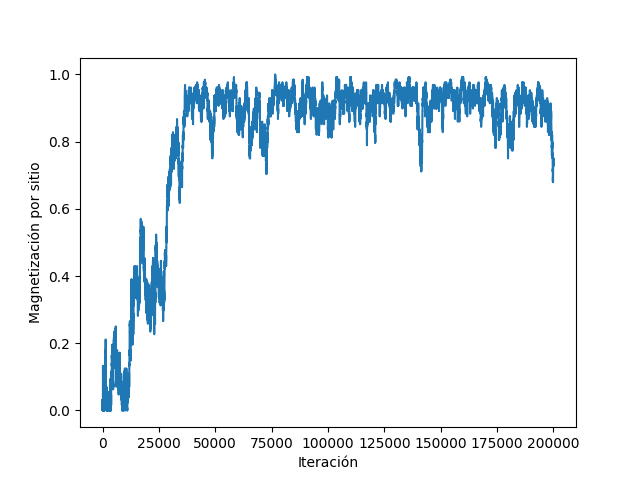
\includegraphics[scale=.6]{./figuras/equil_mag.png}\par}
\end{mdframed}



\section{Longitud de Correlación}

Otra característica distintiva de las transiciones de fase de 2do orden es el desarrollo de
correlaciones de largo rango dentro del sistema. Para estudiar este fenómeno
consideramos la función:
\begin{equation}
    C(\bar r_1, \bar r_2) = \mean{S_1 S_2} - \mean{S_1}\mean{S_2},
\end{equation}
que expresa la correlación entre un spin en la posición $\bar r_1$ y otro en la
posición $\bar r_2$.
Dada la simetría del sistema, en nuestro caso
esta función solo puede depender de la variable $R=|\bar r_1 - \bar r_2|$. Para
sistemas que tienen interacciones locales y a altas temperaturas








\end{document}


